\subsection{Intelligence artificielle}
    \subsubsection{NPC Zone \& Système de déplacement}
    Nous avons essayé plusieurs types de déplacement pour les IA. Nous avons fait des NPC zones qui permettent de créer des quartiers
    où les NPC peuvent se balader librement dans la zone. Si un NPC est tué dans la zone, un nouveau apparait avec un effet visuel 
    approprié (shader d'apparition).
    \newline
    
    Pour le système de déplacement de l'IA,
    nous avons essayé plusieurs algorithmes différents :\newline
    
    \begin{itemize}
        \item Le premier algorithme que nous avions montré lors de la première soutenance
        était un déplacement vers un élément alétoire d'une liste de coordonnées prédéfinie.
        Le tracé était de ce fait trop prévisible et ne permettait pas de se déplacer librement en restant discret.
        De plus, si un personnage allait d'un point A vers un point B, et un autre de B vers A,
        alors prenant le chemin le plus court ils finissaient par se croiser (face à face) et finir coincés.
        \newline
        \item Nous avons donc décidé de rajouter plus d'aléatoire dans leurs déplacements.
        Les IA cherchent une destination "accessible" dans un rayon proche.
        Le problème était que la librairie Unity AI intégrée cherche un chemin complet ou partiel.
        Le rendu final montrait des personnages qui finissaient toujours par être attirés par les bordures de la carte.
        \newline

        \item  Le dernier système intégré cherche une destination dans une certaine zone.
        Au lieu de chercher un point proche de lui, il cherche un chemin vers une destination aléatoire, 
        et recommence lorsque ce point est atteint ou si aucun chemin complet n'a été trouvé.

        
        \begin{figure}[hbt!]
            \centering
            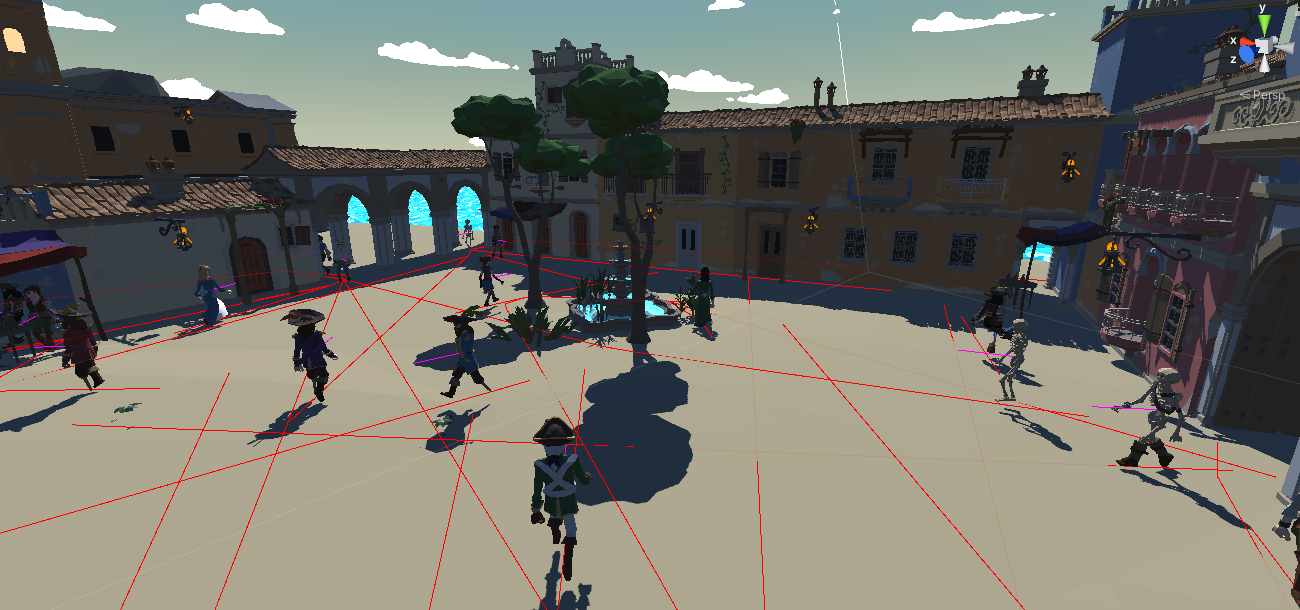
\includegraphics[scale=0.43]{navmesh_path.png}
            \caption{Représentation vectorielle des path des IA}
        \end{figure}
    

    \end{itemize}
    
   
    \subsubsection{Evenements}

    Afin de rendre les IA moins scriptées, nous avons ajouté des événements aléatoires.
    
    En outre, des zones de discussion ont été implémentées : ce sont des zones où les joueurs et le NPC peuvent interagir 
    et se fondre dans la discussion pour se cacher. Les IA qui les traversent s'y arrêtent, parlent,avant de repartir au bout d'une durée 
    de temps aléatoire.

    \begin{figure}[hbt!]
        \centering
        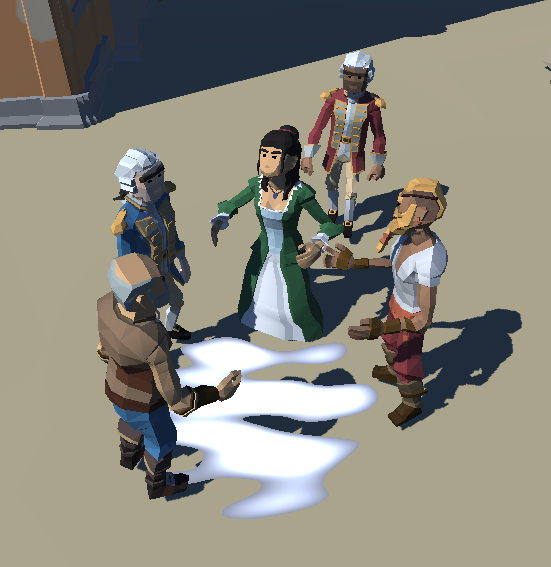
\includegraphics[scale=0.5]{talk_zone.png}
        \caption{Zone de discussion}
    \end{figure}